\documentclass[12pt]{article}
% Revised September 22, 2026.
% PDF reproduction: compile to the corresponding public/pdfs path, then run
% python scripts/stamp-pdf-revisions.py in the website checkout (pypdf, reportlab).
% This adds only a first-page margin date; it does not reflow mathematical content.

\usepackage[T1]{fontenc}
\usepackage[utf8]{inputenc}
\usepackage[margin=1in]{geometry}
\usepackage{amsmath,amssymb,amsthm,mathtools}
\usepackage{microtype}
\usepackage{mathpazo}
\usepackage{xcolor}
\usepackage{tikz}
\usetikzlibrary{arrows.meta,positioning,calc,decorations.pathreplacing}
\usepackage[colorlinks=true,linkcolor=blue!60!black,citecolor=blue!60!black,urlcolor=blue!60!black]{hyperref}

\newtheorem{theorem}{Theorem}
\newtheorem{proposition}[theorem]{Proposition}
\newtheorem{lemma}[theorem]{Lemma}
\newtheorem{corollary}[theorem]{Corollary}
\newtheorem{remark}[theorem]{Remark}
\newtheorem{example}[theorem]{Example}

\newcommand{\Galois}{\operatorname{Gal}}

\title{\textbf{A Galois-Theoretic and Frobenius-Descent Viewpoint\\ on a Polynomial Composition Law}}
\author{Henry Shin}
\date{}

\begin{document}
\maketitle

\begin{abstract}
This note gives a second proof of a polynomial composition criterion for separated polynomial differences.  The guiding principle is that if
\[
    F(x)-G(y) \mid P(x)-Q(y)
\]
in \(k[x,y]\), then the functions \(P\) and \(Q\) are constant on the generic fibers of \(F\) and \(G\), respectively.  In the separable case this can be made literal using the Galois group of the generic fiber.  In positive characteristic, the remaining inseparable cases are removed by a Frobenius descent argument.  The result is a characteristic-free proof of the full separated composition theorem, together with an explicit division algorithm for recovering the outer polynomial.
\end{abstract}

\section{Introduction}

A useful algebraic rigidity phenomenon is the following: if one separated polynomial difference divides another separated polynomial difference, then the outer polynomials must come from a common composition.  In its most symmetric form this says that, for a nonconstant \(g\in k[t]\),
\[
    g(x)-g(y)\mid f(x)-f(y)
    \qquad\Longleftrightarrow\qquad
    f=h\circ g
\]
for some \(h\in k[t]\).  The forward implication is the interesting direction.

The free-module proof of this result is very efficient: one expands \(k[x,y]\) as a finite free module over \(k[F(x),G(y)]\) and compares coefficients in a residue rectangle.  The purpose of this note is to present a complementary viewpoint.  The Galois-theoretic proof says that, over the generic value \(T\), all points in the fiber of \(F\) must have the same \(P\)-value, and all points in the fiber of \(G\) must have the same \(Q\)-value.  Therefore these values descend to a rational function of \(T\); integrality upgrades that rational function to a polynomial.

This method initially appears to require separability, namely \(F'\neq 0\) and \(G'\neq 0\).  The main point developed below is that this is not a real limitation.  If an inner polynomial has zero derivative, then the divisibility condition forces the corresponding outer polynomial to have zero derivative as well.  Both polynomials then descend through the Frobenius map, and induction reduces the problem to the separable case.

\begin{remark}[Relation with reducibility questions]
This criterion is close in spirit to classical and modern questions about the reducibility of polynomials of the form \(P(x)-Q(y)\).  The theorem here does not classify all possible factors of \(P(x)-Q(y)\).  Rather, it handles the special but important situation in which a prescribed factor is itself separated, namely \(F(x)-G(y)\).  In that case the divisibility is strong enough to force actual composition.
\end{remark}

\section{The main theorem}

\begin{theorem}[Separated composition criterion]\label{thm:main}
Let \(k\) be a field, and let
\[
    F,G,P,Q\in k[t]
\]
with
\[
    \deg F>0,\qquad \deg G>0.
\]
If
\[
    F(x)-G(y)\mid P(x)-Q(y)
\]
in \(k[x,y]\), then there exists a polynomial \(S\in k[t]\) such that
\[
    P(t)=S(F(t)),
    \qquad
    Q(t)=S(G(t)).
\]
Conversely, if such an \(S\) exists, then
\[
    F(x)-G(y)
    \mid
    P(x)-Q(y).
\]
\end{theorem}

The converse follows immediately from the universal identity
\[
    U-V \mid S(U)-S(V)
\]
in \(k[U,V]\).  The rest of the note proves the forward implication.

The symmetric composition criterion is obtained by taking \(F=G=g\) and \(P=Q=f\).

\begin{corollary}[Symmetric form]\label{cor:symmetric}
Let \(g\in k[t]\) be nonconstant, and let \(f\in k[t]\). Then
\[
    g(x)-g(y)\mid f(x)-f(y)
\]
in \(k[x,y]\) if and only if there exists \(h\in k[t]\) such that
\[
    f(t)=h(g(t)).
\]
\end{corollary}

\section{The separable generic-fiber argument}

We first prove Theorem \ref{thm:main} under the additional hypotheses
\[
    F'\neq 0,
    \qquad
    G'\neq 0.
\]
This is the part where Galois theory enters.

\begin{lemma}[Separable generic fiber]\label{lem:separable-generic-fiber}
Let \(R\in k[t]\) be nonconstant and suppose \(R'\neq 0\).  Let \(T\) be an indeterminate. Then
\[
    R(Z)-T\in k(T)[Z]
\]
is separable.
\end{lemma}

\begin{proof}
The derivative of \(R(Z)-T\) with respect to \(Z\) is \(R'(Z)\).  If \(R(Z)-T\) had a multiple root \(\alpha\) in an algebraic closure of \(k(T)\), then
\[
    R(\alpha)=T,
    \qquad
    R'(\alpha)=0.
\]
Since \(R'\) is a nonzero polynomial over \(k\), the equation \(R'(\alpha)=0\) would make \(\alpha\) algebraic over \(k\).  Then \(R(\alpha)\) would also be algebraic over \(k\), contradicting the transcendence of \(T\).  Hence \(R(Z)-T\) has no multiple root.
\end{proof}

\begin{proposition}[The separable case]\label{prop:separable-case}
Assume
\[
    F'\neq 0,
    \qquad
    G'\neq 0.
\]
If
\[
    F(x)-G(y)\mid P(x)-Q(y)
\]
in \(k[x,y]\), then there exists \(S\in k[t]\) such that
\[
    P=S\circ F,
    \qquad
    Q=S\circ G.
\]
\end{proposition}

\begin{proof}
Let \(T\) be an indeterminate and set
\[
    K=k(T).
\]
By Lemma \ref{lem:separable-generic-fiber}, both
\[
    F(X)-T,
    \qquad
    G(Y)-T
\]
are separable over \(K\).  Let \(L\) be a common splitting field over \(K\) for their product, so \(L/K\) is finite Galois.  Choose roots
\[
    \alpha\in L,
    \qquad
    \beta\in L
\]
such that
\[
    F(\alpha)=T,
    \qquad
    G(\beta)=T.
\]

By hypothesis there exists \(H(x,y)\in k[x,y]\) with
\[
    P(x)-Q(y)=\bigl(F(x)-G(y)\bigr)H(x,y).
\]
Evaluating at \((x,y)=(\alpha,\beta)\) gives
\[
    P(\alpha)=Q(\beta).
\]

Now let \(\sigma\in \Galois(L/K)\).  Since \(\sigma\) fixes \(T\), we have
\[
    F(\sigma(\alpha))=\sigma(F(\alpha))=\sigma(T)=T.
\]
Thus \(\sigma(\alpha)\) is another point of the generic fiber of \(F\).  Evaluating the divisibility identity at \((x,y)=(\sigma(\alpha),\beta)\) gives
\[
    P(\sigma(\alpha))-Q(\beta)
    =
    \bigl(F(\sigma(\alpha))-G(\beta)\bigr)H(\sigma(\alpha),\beta)
    =0.
\]
Therefore
\[
    P(\sigma(\alpha))=Q(\beta)=P(\alpha).
\]
Since the coefficients of \(P\) lie in \(k\subseteq K\),
\[
    \sigma(P(\alpha))=P(\sigma(\alpha))=P(\alpha).
\]
Hence \(P(\alpha)\) is fixed by the full Galois group \(\Galois(L/K)\), and so
\[
    P(\alpha)\in K=k(T).
\]

We now improve this rational function to a polynomial.  Write the leading coefficient of \(F\) as \(a\in k^\times\).  The element \(\alpha\) satisfies the monic equation
\[
    Z^{\deg F}+\cdots+a^{-1}(F(0)-T)=0
\]
over \(k[T]\).  Thus \(\alpha\) is integral over \(k[T]\), and therefore \(P(\alpha)\) is integral over \(k[T]\).  Since \(k[T]\) is integrally closed and
\[
    P(\alpha)\in k(T),
\]
we get
\[
    P(\alpha)\in k[T].
\]
So there exists \(S(T)\in k[T]\) such that
\[
    P(\alpha)=S(T).
\]

Because \(T=F(\alpha)\), this says
\[
    P(\alpha)=S(F(\alpha)).
\]
The element \(\alpha\) is transcendental over \(k\): otherwise \(T=F(\alpha)\) would be algebraic over \(k\), impossible.  Hence the polynomial identity
\[
    P(t)=S(F(t))
\]
holds in \(k[t]\).

Finally,
\[
    Q(\beta)=P(\alpha)=S(T)=S(G(\beta)).
\]
The same transcendence argument for \(\beta\) gives
\[
    Q(t)=S(G(t)).
\]
This proves the separable case.
\end{proof}

\begin{figure}[htbp]
\centering
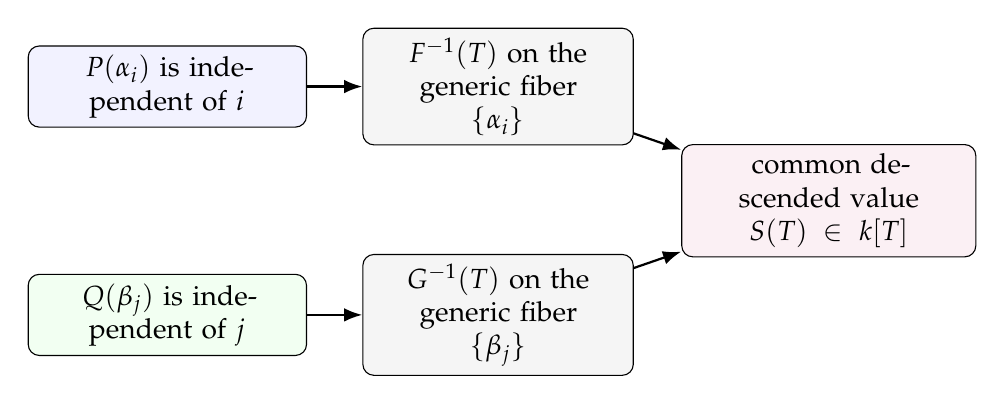
\begin{tikzpicture}[>=Latex]
    \node[draw,rounded corners,align=center,fill=blue!5,text width=3.3cm]
        (Pbox) at (-3.4,1.45) {\(P(\alpha_i)\) is independent of \(i\)};
    \node[draw,rounded corners,align=center,fill=green!5,text width=3.3cm]
        (Qbox) at (-3.4,-1.45) {\(Q(\beta_j)\) is independent of \(j\)};

    \node[draw,rounded corners,align=center,fill=gray!8,text width=3.2cm]
        (Ffib) at (0.8,1.45) {\(F^{-1}(T)\) on the generic fiber\\ \(\{\alpha_i\}\)};
    \node[draw,rounded corners,align=center,fill=gray!8,text width=3.2cm]
        (Gfib) at (0.8,-1.45) {\(G^{-1}(T)\) on the generic fiber\\ \(\{\beta_j\}\)};

    \node[draw,rounded corners,align=center,fill=purple!6,text width=3.5cm]
        (base) at (5.0,0) {common descended value\\ \(S(T)\in k[T]\)};

    \draw[->,thick] (Pbox) -- (Ffib);
    \draw[->,thick] (Qbox) -- (Gfib);
    \draw[->,thick] (Ffib) -- (base);
    \draw[->,thick] (Gfib) -- (base);
\end{tikzpicture}
\caption{The separable proof: the divisibility identity forces \(P\) and \(Q\) to be constant on the generic fibers.  Galois invariance gives a rational function of \(T\), and integrality upgrades it to a polynomial.}
\end{figure}

\section{Frobenius descent removes the derivative hypotheses}

We now handle the inseparable cases in positive characteristic.  The basic observation is that if an inner polynomial has zero derivative, then the divisibility condition forces the corresponding outer polynomial to have zero derivative as well.

\begin{lemma}[Zero derivative and Frobenius form]\label{lem:zero-derivative}
Let \(k\) have characteristic \(p>0\).  For \(R\in k[t]\),
\[
    R'(t)=0
\]
if and only if there exists a unique \(R_1\in k[t]\) such that
\[
    R(t)=R_1(t^p).
\]
\end{lemma}

\begin{proof}
Write
\[
    R(t)=\sum_{n\geq 0}a_n t^n.
\]
Then
\[
    R'(t)=\sum_{n\geq 1} n a_n t^{n-1}.
\]
In characteristic \(p\), the coefficient \(n a_n\) vanishes automatically when \(p\mid n\).  Thus \(R'=0\) exactly when \(a_n=0\) for every exponent \(n\) not divisible by \(p\).  Equivalently,
\[
    R(t)=\sum_{m\geq 0}a_{pm}t^{pm}=R_1(t^p),
\]
where
\[
    R_1(u)=\sum_{m\geq 0}a_{pm}u^m.
\]
\end{proof}

\begin{lemma}[Descent of divisibility through a Frobenius subring]\label{lem:frob-descent}
Assume \(\operatorname{char} k=p>0\).  Let
\[
    A=k[X,y]
    \hookrightarrow
    B=k[x,y]
\]
be the inclusion defined by
\[
    X\longmapsto x^p,
    \qquad
    y\longmapsto y.
\]
If \(D,E\in A\), \(D\neq 0\), and \(D\mid E\) in \(B\), then \(D\mid E\) already in \(A\).

The analogous statement holds for the inclusion \(k[x,Y]\hookrightarrow k[x,y]\) with \(Y\mapsto y^p\).
\end{lemma}

\begin{proof}
The ring \(B=k[x,y]\) is a free \(A=k[x^p,y]\)-module with basis
\[
    1,x,x^2,\ldots,x^{p-1}.
\]
Suppose
\[
    E=D\Theta
\]
for some \(\Theta\in B\).  Write uniquely
\[
    \Theta=\sum_{r=0}^{p-1}\Theta_r x^r,
    \qquad
    \Theta_r\in A.
\]
Then
\[
    E=D\Theta_0+\sum_{r=1}^{p-1}D\Theta_r x^r.
\]
Since \(E\in A\), the coefficients of \(x^r\) for \(1\leq r\leq p-1\) must vanish.  Because \(A\) is a domain and \(D\neq0\), this gives
\[
    \Theta_r=0
    \qquad
    (1\leq r\leq p-1).
\]
Thus \(\Theta=\Theta_0\in A\), so \(D\mid E\) in \(A\).
\end{proof}

\begin{proposition}[Frobenius reduction step]\label{prop:frob-step}
Assume \(\operatorname{char} k=p>0\).  Suppose
\[
    F(x)-G(y)\mid P(x)-Q(y)
\]
in \(k[x,y]\), with \(F,G\) nonconstant.

If \(F'=0\), then \(P'=0\).  Writing
\[
    F(t)=F_1(t^p),
    \qquad
    P(t)=P_1(t^p),
\]
one has
\[
    F_1(X)-G(y)
    \mid
    P_1(X)-Q(y)
\]
in \(k[X,y]\).

Similarly, if \(G'=0\), then \(Q'=0\), and writing
\[
    G(t)=G_1(t^p),
    \qquad
    Q(t)=Q_1(t^p),
\]
one has
\[
    F(x)-G_1(Y)
    \mid
    P(x)-Q_1(Y)
\]
in \(k[x,Y]\).
\end{proposition}

\begin{proof}
We prove the statement for \(F\); the statement for \(G\) is symmetric.

Assume \(F'=0\).  Choose \(H\in k[x,y]\) such that
\[
    P(x)-Q(y)=\bigl(F(x)-G(y)\bigr)H(x,y).
\]
Differentiate with respect to \(x\).  Since \(F'=0\), we get
\[
    P'(x)=\bigl(F(x)-G(y)\bigr)\frac{\partial H}{\partial x}(x,y).
\]
Thus \(F(x)-G(y)\) divides \(P'(x)\) in \(k[x,y]\).  But \(G\) is nonconstant, so \(F(x)-G(y)\) has positive degree in \(y\).  A nonzero polynomial depending only on \(x\) cannot be divisible by a polynomial of positive \(y\)-degree.  Hence
\[
    P'(x)=0.
\]

By Lemma \ref{lem:zero-derivative}, there exist \(F_1,P_1\in k[t]\) such that
\[
    F(t)=F_1(t^p),
    \qquad
    P(t)=P_1(t^p).
\]
Set \(X=x^p\).  Then
\[
    F(x)-G(y)=F_1(X)-G(y)
\]
and
\[
    P(x)-Q(y)=P_1(X)-Q(y).
\]
These two polynomials belong to \(A=k[X,y]\).  Since divisibility holds after embedding \(A\hookrightarrow k[x,y]\), Lemma \ref{lem:frob-descent} shows that it already holds in \(A\).  Therefore
\[
    F_1(X)-G(y)
    \mid
    P_1(X)-Q(y)
\]
in \(k[X,y]\).
\end{proof}

\begin{proof}[Proof of Theorem \ref{thm:main}]
We prove the forward implication by induction on
\[
    N=\deg F+\deg G.
\]
If
\[
    F'\neq0
    \qquad\text{and}\qquad
    G'\neq0,
\]
then Proposition \ref{prop:separable-case} proves the result.

Otherwise, at least one of \(F'\) and \(G'\) is zero.  This can occur only in positive characteristic.  Suppose first that \(F'=0\).  By Proposition \ref{prop:frob-step}, we may write
\[
    F(t)=F_1(t^p),
    \qquad
    P(t)=P_1(t^p),
\]
and we have
\[
    F_1(X)-G(y)
    \mid
    P_1(X)-Q(y)
\]
in \(k[X,y]\).  Since
\[
    \deg F_1=\frac{\deg F}{p}<\deg F,
\]
the induction hypothesis gives a polynomial \(S\in k[t]\) such that
\[
    P_1(t)=S(F_1(t)),
    \qquad
    Q(t)=S(G(t)).
\]
Substituting \(t^p\) into the first identity gives
\[
    P(t)=P_1(t^p)=S(F_1(t^p))=S(F(t)).
\]
Thus
\[
    P=S\circ F,
    \qquad
    Q=S\circ G.
\]

If instead \(G'=0\), the symmetric argument reduces \(G\) and \(Q\) through Frobenius and again applies induction.  The induction terminates because the positive integer \(\deg F+\deg G\) strictly decreases at every inseparable reduction step.
\end{proof}

\begin{figure}[htbp]
\centering
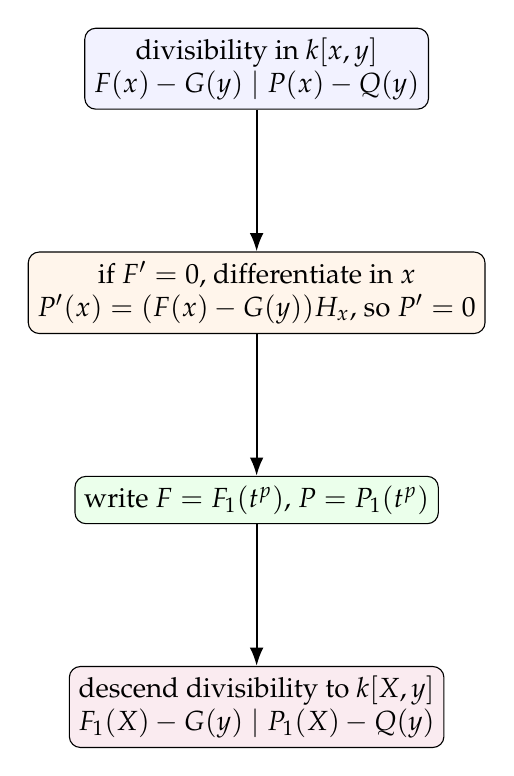
\begin{tikzpicture}[node distance=1.8cm,>=Latex]
    \node[draw,rounded corners,fill=blue!5,align=center] (top) {divisibility in \(k[x,y]\)\\ \(F(x)-G(y)\mid P(x)-Q(y)\)};
    \node[draw,rounded corners,fill=orange!8,below=of top,align=center] (deriv) {if \(F'=0\), differentiate in \(x\)\\ \(P'(x)=(F(x)-G(y))H_x\), so \(P'=0\)};
    \node[draw,rounded corners,fill=green!8,below=of deriv,align=center] (frob) {write \(F=F_1(t^p)\), \(P=P_1(t^p)\)};
    \node[draw,rounded corners,fill=purple!8,below=of frob,align=center] (desc) {descend divisibility to \(k[X,y]\)\\ \(F_1(X)-G(y)\mid P_1(X)-Q(y)\)};
    \draw[->,thick] (top) -- (deriv);
    \draw[->,thick] (deriv) -- (frob);
    \draw[->,thick] (frob) -- (desc);
\end{tikzpicture}
\caption{The Frobenius reduction step.  Inseparability of an inner polynomial forces inseparability of the corresponding outer polynomial, allowing both to descend through \(t\mapsto t^p\).}
\end{figure}

\section{Algorithmic extraction of the outer polynomial}

Once composition is known, the outer polynomial can be recovered by a single polynomial division.

\begin{proposition}[Division algorithm for extracting the outer polynomial]\label{prop:algorithm}
Let \(g,f\in k[t]\), with \(g\) nonconstant.  Let \(S,T\) be indeterminates.  Divide \(f(T)\) by \(g(T)-S\) as a polynomial in \(T\) over \(k[S]\):
\[
    f(T)=A(T,S)\bigl(g(T)-S\bigr)+R(T,S),
    \qquad
    \deg_T R<\deg g.
\]
This division is valid in \(k[S][T]\), since the leading coefficient of \(g(T)-S\) is a unit in \(k[S]\).

Then
\[
    f(t)=h(g(t))
\]
for some \(h\in k[t]\) if and only if the remainder \(R(T,S)\) is independent of \(T\).  In that case
\[
    R(T,S)=h(S).
\]
\end{proposition}

\begin{proof}
If \(f=h\circ g\), then
\[
    f(T)=h(g(T)).
\]
The universal identity
\[
    U-V\mid h(U)-h(V)
\]
gives
\[
    g(T)-S\mid h(g(T))-h(S).
\]
Thus
\[
    f(T)=A(T,S)(g(T)-S)+h(S)
\]
for some \(A(T,S)\in k[S,T]\).  Since \(h(S)\) is independent of \(T\) and \(\deg g>0\), uniqueness of the division algorithm gives
\[
    R(T,S)=h(S).
\]

Conversely, if the remainder is independent of \(T\), say \(R(T,S)=r(S)\), then substituting \(S=g(T)\) into the division identity yields
\[
    f(T)=r(g(T)).
\]
Thus \(f=r\circ g\).
\end{proof}

\begin{example}
Let
\[
    g(T)=T^3+T,
    \qquad
    f(T)=T^6+2T^4+T^2=(T^3+T)^2.
\]
Dividing by \(g(T)-S=T^3+T-S\), we get
\[
    f(T)=(T^3+T+S)(T^3+T-S)+S^2.
\]
The remainder is \(S^2\), so the extracted outer polynomial is
\[
    h(S)=S^2.
\]
\end{example}

\section{Application: a symmetric functional equation}

We now record a concrete application of Corollary \ref{cor:symmetric}.  The square-root notation below is shorthand for working in an algebraic closure of the rational function field \(k(x)\).

\begin{proposition}\label{prop:functional-equation}
Let \(k\) be a field with \(\operatorname{char}k\neq2\), and let \(f\in k[t]\).  Suppose that, in an algebraic closure of \(k(x)\),
\[
    f(x)
    =
    f\left(\frac{-x+\sqrt{-3x^2-4}}{2}\right)
    =
    f\left(\frac{-x-\sqrt{-3x^2-4}}{2}\right).
\]
Then there exists \(h\in k[t]\) such that
\[
    f(t)=h(t^3+t).
\]
\end{proposition}

\begin{proof}
Let
\[
    u_+=\frac{-x+\sqrt{-3x^2-4}}{2},
    \qquad
    u_-=\frac{-x-\sqrt{-3x^2-4}}{2}.
\]
These are the two roots of
\[
    Y^2+xY+x^2+1=0
\]
over \(k(x)\).  We have the factorization
\[
    Y^3+Y-(x^3+x)
    =
    (Y-x)(Y^2+xY+x^2+1).
\]
Thus the three roots of
\[
    Y^3+Y-(x^3+x)
\]
are
\[
    x,
    \qquad
    u_+,
    \qquad
    u_-.
\]
They are distinct in an algebraic closure of \(k(x)\): the two quadratic roots are distinct because \(-3x^2-4\) is not the zero rational function when \(\operatorname{char}k\neq2\), and neither quadratic root equals \(x\), since that would force \(3x^2+1=0\) as a rational function.

By hypothesis,
\[
    f(Y)-f(x)
\]
vanishes at all three roots of \(Y^3+Y-(x^3+x)\).  Therefore
\[
    Y^3+Y-(x^3+x)
    \mid
    f(Y)-f(x)
\]
in \(k(x)[Y]\).  Since \(Y^3+Y-(x^3+x)\) is monic in \(Y\), Gauss's lemma gives the divisibility already in \(k[x,Y]\):
\[
    (Y^3+Y)-(x^3+x)
    \mid
    f(Y)-f(x).
\]
Applying Corollary \ref{cor:symmetric} to
\[
    g(t)=t^3+t
\]
gives
\[
    f(t)=h(g(t))=h(t^3+t)
\]
for some \(h\in k[t]\).
\end{proof}

\begin{remark}
No assumption \(\operatorname{char}k\neq3\) is needed.  If \(\operatorname{char}k=3\), then
\[
    (t^3+t)'=1,
\]
so the generic fiber of \(t^3+t\) is separable.  The exclusion of characteristic \(2\) is only needed for the displayed branch formula with division by \(2\).
\end{remark}

\section{What this viewpoint proves}

The Galois argument proves the theorem cleanly when the generic fibers are separable.  The Frobenius descent step shows that this is not merely a separable-characteristic trick: it gives the full theorem over an arbitrary field.

It is useful to separate two related but different problems:

\begin{enumerate}
    \item The theorem of this note asks: if a specific separated polynomial
    \[
        F(x)-G(y)
    \]
    divides
    \[
        P(x)-Q(y),
    \]
    what follows?  The answer is complete: \(P\) and \(Q\) come from one polynomial \(S\) by composition.

    \item The broader reducibility problem asks: when does
    \[
        P(x)-Q(y)
    \]
    have any nontrivial factor at all? That is much deeper. One source of reducibility is a common outer composition
    \[
        P=R\circ \widetilde P,
        \qquad
        Q=R\circ \widetilde Q,
    \]
    where \(\deg R>1\) and both inner polynomials are nonconstant. Then \(\widetilde P(x)-\widetilde Q(y)\) is a proper nonconstant factor of \(P(x)-Q(y)\). Classifying other possibilities leads into the theory of Fried, Cassels, Ritt-type decompositions, and the Davenport--Lewis--Schinzel problem.
\end{enumerate}

Thus the present theorem is not a complete irreducibility criterion for \(P(x)-Q(y)\).  It is instead a rigidity theorem for separated factors.  Its strength is that once the factor has the special form \(F(x)-G(y)\), the conclusion is exact and characteristic-free.

\begin{thebibliography}{9}

\bibitem{TaoMO}
Terry Tao,
\emph{When is \(P(x)-Q(y)\) irreducible?},
MathOverflow, 2012.
\url{https://mathoverflow.net/questions/105747/when-is-px-qy-irreducible}

\bibitem{DaoMO}
Hailong Dao,
\emph{Irreducibility of polynomials in two variables},
MathOverflow, 2010.
See especially Graham Leuschke's answer discussing the Fried--Cassels classification result for indecomposable polynomials over \(\mathbb C\).
\url{https://mathoverflow.net/questions/14076/irreducibility-of-polynomials-in-two-variables}

\end{thebibliography}

\end{document}
